\documentclass[11pt,a4paper]{article}

\usepackage[utf8]{inputenc}
\usepackage[T1]{fontenc}
\usepackage{lmodern}
\usepackage{microtype}
\usepackage[margin=1in]{geometry}
\usepackage{amsmath,amssymb,amsthm}
\usepackage{graphicx}
\usepackage{booktabs}
\usepackage{array}
\usepackage{caption}
\usepackage{subcaption}
\usepackage{hyperref}
\usepackage{natbib}
\usepackage{xcolor}
\usepackage{setspace}
\usepackage{float}

\hypersetup{
  colorlinks=true,
  linkcolor=blue!50!black,
  citecolor=blue!50!black,
  urlcolor=blue!50!black
}

\setlength{\parindent}{0pt}
\setlength{\parskip}{6pt}

\title{Architectural Variance Dominates Stimulus Variance in\\Six of Seven Substrate-Agnostic Consciousness Operationalizations\\[6pt]
\large{A cross-substrate comparison with human fMRI BOLD reveals coincidental magnitude alignment of fundamentally different variance sources}}

\author{Nate Travis\\[3pt]
\textit{Devmance Labs}\\
\texttt{labs@devmance.com}}

\date{\today}

\begin{document}
\maketitle

\begin{abstract}
\noindent
Mathematical theories of consciousness --- Integrated Information Theory (IIT), Global Workspace Theory (GWT), Attention Schema Theory (AST), Higher-Order Thought (HOT), Predictive Processing Theory (PPT), Quantum Information Theory (QIT), and the Free Energy Principle (FEP) --- are commonly framed as substrate-independent: identical mathematics applied to any sufficiently structured dynamical system. If this substrate-independence carries empirical content, the theories should produce concordant per-stimulus scores when applied to different physical substrates processing the same input. We test this by defining a substrate-agnostic operationalization of all seven theories that takes only an activity matrix ($T$ timesteps $\times$ $N$ nodes), implementing identical calculator code, and applying it to (a) attention activations from four open-weight transformer language models reading narrative stories and (b) functional MRI BOLD signals from three subjects listening to the same stories \citep{lebel2023natural}. The seven operationalizations are author-defined substrate-portable surrogates of each theory: single-formula calculators of $(T \times N)$ activity, not reproductions of each theory's published computational definition (most of which are not substrate-portable in their original form --- IIT 3.0 is computationally intractable above $\sim$10 nodes, GWT and AST are non-algorithmic theoretical frameworks, and the others have no canonical algorithm on fMRI BOLD or transformer activations). Cross-substrate null results therefore bear on the surrogates, not directly on the published theories.

At the population level, AI and human substrate distributions overlap for several theories (unified-score gap $=-1.7$ points on a 0--100 scale; three theories show sub-5-point gaps). The magnitude-alignment pattern has been interpreted in prior behavioral work as evidence that consciousness theories cannot discriminate AI from humans. Variance decomposition complicates that interpretation: \emph{human} substrate variance is stimulus-driven (between-story SD $>$ within-subject SD), while \emph{AI} substrate variance is architecturally-driven (between-model SD $>$ between-story SD for six of seven theories). The population-level magnitude alignment is consistent with coincidental overlap of fundamentally different variance sources rather than measurement of a substrate-shared phenomenon.

When within-substrate noise is averaged out, six of seven theories show no detectable cross-substrate per-stimulus correlation (Pearson $r \in [-0.17, +0.18]$, all permutation $p > 0.1$). Global Workspace Theory shows the strongest signal (model-and-subject-averaged $r=+0.365$, permutation $p=0.001$, split-half stable), but per-architecture breakdown ($r$ in $[-0.19, +0.43]$ across four AI models, with only one architecture above $+0.4$) is consistent with the across-architecture variation being noise at $n=4$. Fisher-Rao information-geometric integration produces a Riemannian-mean cross-substrate $r=-0.185$ ($p=0.11$), stable across alternative prior matrices (range $[-0.21, -0.16]$ over uniform, identity, and 20 random perturbations of the literature-based compatibility prior).

The substrate-independence claim of contemporary consciousness theory, as standardly operationalized, is not testable by these operationalizations on current AI substrates: six of seven theories produce AI-side outputs whose per-stimulus variation is dominated by architectural noise, leaving no detectable stimulus-driven measurement to compare against the human-side stimulus-driven measurement. Mathematical consciousness theories cannot serve as cross-substrate discriminators here not because AI and humans look the same to them, but because the theories' AI-side measurements do not track stimulus content sufficient to test the question. Whether stimulus-relevant signal exists in the AI substrate but is invisible to these operationalizations, or no such signal exists at all, the present data do not decide. GWT shows the strongest cross-substrate signal among the seven, but the per-architecture pattern (only one of four AI architectures exceeding $r=+0.4$) is consistent with statistical noise at $n=4$ architectures.

\vspace{6pt}
\noindent\textbf{Code and data:} \url{https://github.com/devmance/SEMCA}
\end{abstract}

\section{Introduction}

Mathematical theories of consciousness --- IIT \citep{tononi2004information}, GWT \citep{baars1988cognitive,dehaene2001towards}, AST \citep{graziano2013consciousness}, HOT \citep{rosenthal1986two}, PPT \citep{clark2013whatever,hohwy2013predictive}, the Free Energy Principle \citep{friston2010free}, and quantum-informational frameworks \citep{hameroff1996orchestrated,tegmark2014consciousness} --- are commonly advanced as substrate-independent. Each is framed as a mathematical claim about dynamical systems with appropriate causal-informational structure, applying regardless of the substrate that implements that structure. Substrate-independence is what makes empirical questions about AI consciousness tractable in principle: if the theories give substrate-portable measurements, we can apply them to any system that exposes the right kind of activity.

A natural empirical test of substrate-independence is direct cross-substrate comparison: define one mathematical operationalization, apply it identically to two substrates processing the same input, ask whether the resulting scores agree. Behavioral approximations of this test --- comparing the theories' implicit behavioral predictions on humans and on contemporary large language models --- have suggested that the theories produce similar scores across the two populations. This has been read as supporting a kind of ``no-discrimination'' finding: humans and AI score in overlapping ranges, so the theories cannot serve as consciousness discriminators.

We argue this reading is too quick. The behavioral comparisons compare \emph{behavioral signatures} (text outputs), not the theories' substrate-level operationalizations. They tell us how the theories' predicted behavioral surfaces look on different systems but say nothing about whether the theories' underlying mathematics, applied directly to substrate activity, produces shared or divergent measurements. The most-cited substrate-level cross-system consciousness measurement to date is the Perturbational Complexity Index (PCI) of \citet{casali2013theoretically}, which characterizes brain-state complexity from TMS-EEG perturbation responses and discriminates conscious from unconscious states within a single substrate type. A direct cross-substrate test --- applying the same mathematical operationalization to two physically different substrates on the same input --- would either strengthen the no-discrimination finding (substrate-level measurements also fail to discriminate) or sharply complicate it (substrate measurements discriminate even when behavior does not).

We perform that direct substrate-level test. We define an abstract \texttt{Substrate} as a dynamical system observable as an activity matrix of dimensions ($T \times N$) --- $T$ timesteps $\times$ $N$ nodes, real-valued activations --- and implement substrate-agnostic operationalizations of all seven theories on this representation. Transformer attention activations and human fMRI BOLD signals both fit this abstraction, and we apply identical mathematics to each on the same stimulus set (76 narrative stories from \citealt{lebel2023natural}). The key analyses are:

\begin{enumerate}
  \item \textbf{Population-level magnitude comparison} --- does each theory's pooled distribution of AI scores overlap with its pooled distribution of human scores?
  \item \textbf{Per-stimulus cross-substrate correlation} --- averaging within-substrate noise out, does the same theory rank stimuli the same way across substrates?
  \item \textbf{Variance decomposition on the AI side} --- for each theory, is per-story variance dominated by \emph{which stimulus} (substrate-shared signal) or \emph{which model} (substrate-blind noise)?
\end{enumerate}

Three findings emerge:

\begin{itemize}
  \item Population magnitudes overlap substantially across substrates.
  \item Per-stimulus correlations are essentially zero for six of seven theories; only GWT shows a detectable cross-substrate signal, and that signal is architecture-dependent.
  \item For six of seven theories, the AI substrate's per-story variance is dominated by architecture (which model is running), not stimulus (which story is being processed). The substrate-agnostic operationalizations, when run on transformer activations, produce stimulus-insensitive outputs whose per-story differences reflect architectural noise.
\end{itemize}

For six of seven operationalizations, the theories' AI-side outputs do not measure anything stimulus-relevant --- whether because no such signal exists in the activations or because these operationalizations cannot resolve it. The apparent cross-substrate magnitude overlap is consistent with coincidental alignment of architecturally-driven AI variance and stimulus-driven human variance. The substrate-independence claim of contemporary consciousness theory is not testable on current AI substrates by these operationalizations on these stimuli: no AI-side stimulus-driven measurement of sufficient signal-to-noise is available to compare with the human-side measurement.

GWT is a partial exception. Its substrate-agnostic operationalization (cross-group ignition / global broadcast index) does produce stimulus-driven AI-side variation that modestly correlates with human-side stimulus-driven variation ($r=+0.365$ after noise averaging). However, GWT's cross-substrate signal is heterogeneous across the four AI architectures tested, with the strongest correlation driven by one model family. The theory is thus the strongest candidate among the seven for an empirically meaningful substrate-portability claim, but the evidence is preliminary and architecture-dependent.

\section{The Substrate Abstraction and Seven Operationalizations}

\subsection{The substrate}

We define an abstract \texttt{Substrate} as a tuple $\langle A, G, C, \tau \rangle$ where:

\begin{itemize}
  \item $A \in \mathbb{R}^{T \times N}$ is the activity matrix: $T$ discrete timesteps, $N$ nodes, each cell a real-valued activation.
  \item $G \subseteq 2^{[N]}$ is an optional node-group partition (e.g., transformer layers, fMRI functional networks). Groups are used by theories that distinguish within-group from between-group dynamics.
  \item $C \in \mathbb{R}^{N \times N}$ is an optional connectivity matrix (transformer attention or fMRI structural connectivity). Absent $\rightarrow$ fully connected default.
  \item $\tau$ is the substrate type marker, used only to select the prediction adapter (\S\ref{sec:adapters}); no theory calculator branches on substrate type.
\end{itemize}

Two concrete substrates instantiate this abstraction:

\paragraph{Transformer substrate.} For a transformer with multi-head self-attention \citep{vaswani2017attention} consisting of $H$ heads across $K$ layers processing a sequence of length $L$, we set $T = L$ and $N = K \times H$, with $A[t, k \cdot H + h]$ the total attention mass directed to position $t$ at head $h$ of layer $k$. Groups partition by layer ($K$ groups of $H$ heads each). Each attention head is treated as one node and its activity over the sequence as one time series.

\paragraph{fMRI substrate.} For a subject listening to a story, per-sentence evoked BOLD is extracted by averaging voxel activity over a 4-second window beginning 5 seconds after sentence offset (canonical HRF lag plus integration window, after \citealt{boynton1996linear}). Voxels are clustered via $K$-means into $P = 200$ functional parcels; parcels are super-clustered into $K = 10$ functional networks ($G$). $A$ is ($n_{\mathrm{sentences}} \times 200$).

The abstraction is intentionally minimal: any dynamical system expressible as a ($T \times N$) real-valued activity matrix qualifies.

\subsection{Substrate-agnostic theory operationalizations}

We implement each theory as a function \texttt{theory(substrate)} $\rightarrow$ \texttt{score} $\in [0, 100]$. Each operationalization uses no substrate-type-specific information; identical Python code runs on \texttt{TransformerSubstrate} and \texttt{FMRISubstrate}.

Each theory's score on $[0, 100]$ combines two or three sub-scores. The substrate-agnostic operationalizations below are the ones we implement; the published theories themselves admit other operationalizations.

\paragraph{IIT (integrated information).} A node-similarity graph $W[i,j] = \cos(\text{activity}[:,i], \text{activity}[:,j])$ is built from the substrate's activity matrix. For each node-group, we find the Minimum Information Partition (MIP) via Normalized Cut \citep{shi2000normalized} on $W$ restricted to that group; for the system as a whole we compute cross-group $\Phi$ on the group-level super-graph. Three components: \emph{PLG} (per-local-group $\Phi$, mean of within-group $\Phi$), \emph{CGI} (cross-group $\Phi$ on the group-level graph), and \emph{PV} (standard deviation of $\Phi_G$ across groups). The Normalized Cut serves as a tractable surrogate for the full IIT 3.0 algorithm of \citet{oizumi2014phenomenology}, which is computationally intractable above $\sim$10 nodes. Exhaustive bipartition search is used for groups with $\leq 8$ nodes; stratified sampling otherwise. (This induces an algorithmic asymmetry across substrates --- discussed in \S\ref{sec:limitations}.)

\paragraph{GWT (global workspace).} Three sub-scores combined as $0.40 \cdot \text{CGAS} + 0.30 \cdot \text{NDE} + 0.30 \cdot \text{IGC}$. \emph{CGAS} (Cross-Group Activation Spread) is the per-timestep fraction of node-groups whose mean activity exceeds the 85th percentile, averaged over timesteps. \emph{NDE} (Node-Diversity Engagement) is the per-timestep fraction of all nodes above the global 85th-percentile activity quantile. \emph{IGC} (Inter-Group Coupling) is the mean pairwise correlation between group-level activity vectors. The construction targets the substrate-symmetric signature of synchronized broadcast events rather than a Fourier spectral measurement.

\paragraph{AST (attention schema).} Three sub-scores combined as $0.45 \cdot \text{UP} + 0.30 \cdot \text{SC} + 0.25 \cdot \text{SCoh}$. \emph{UP} (Upstream Predictability) is the mean canonical correlation between adjacent node-groups (the top-8 singular values of the cross-covariance, averaged). \emph{SC} (Schema Compression) is the spectral entropy of each group's activity matrix mapped to a compression score ($1 - H / H_{\max}$). \emph{SCoh} (Schema Coherence) is the Frobenius cosine similarity between successive groups' normalized correlation matrices. The operationalization tests whether downstream group behavior is predictable from upstream group behavior in a way that resembles a learned schema.

\paragraph{HOT (higher-order thought).} Three sub-scores: \emph{SRC} (Self-Representation Capacity, mean canonical correlation over all pairs $(G_i, G_j)$ with $i < j$ and within a small group-distance window), \emph{RD} (Recursive Depth, the slope of CCA decay as group-distance grows --- slow decay indicates chains of representational nesting), and \emph{MRS} (Meta-Representation Stability, the cross-temporal-window stability of cross-group CCA patterns). The operationalization tests whether later groups encode information about earlier groups in a manner stable across temporal windows.

\paragraph{PPT (predictive processing).} Requires a prediction adapter (\S\ref{sec:adapters}). Three sub-scores: \emph{PDE} (Prediction-Distribution Entropy, mean per-step entropy of the adapter's predicted-next-state distribution; low entropy = sharp prediction = high confidence), \emph{HPET} (Hierarchical Prediction-Error Trajectory, correlation between group-index and group-level prediction error --- PPT predicts error \emph{decreases} from earlier to later groups), and \emph{PWCE} (Precision-Weighted Cross-Entropy, cross-entropy weighted by precision = inverse of per-step prediction entropy).

\paragraph{QIT (quantum information theory, weak operationalization).} Three sub-scores, following the substrate-portable quantities discussed by \citet{tegmark2014consciousness}: \emph{LRMI} (Long-Range Mutual Information, mutual information between substrate activity vectors at distant \emph{timesteps} --- distances $d \in \{1, 3, 5, 10\}$ are averaged), \emph{CNC} (Cross-Node Coherence, mean pairwise mutual information between sampled node activity vectors), and \emph{BCHSH} (Bell-CHSH-style correlation for selected node pairs under node-group ``measurement settings'', normalized to $[0, 100]$ over the classical-to-quantum range $[0, 2\sqrt{2}]$). Note: LRMI uses temporal separation, not node-index separation; this is a design choice for substrate-symmetric portability, discussed in \S\ref{sec:limitations}.

\paragraph{FEP (free energy principle).} Three sub-scores combined as $0.40 \cdot \text{VFE} + 0.30 \cdot \text{LFED} + 0.30 \cdot \text{AIIG}$. Following \citet{friston2010free}, variational free energy is approximated by the cross-entropy series from the prediction adapter: $\text{VFE}_t \approx -\log p(\text{observed}_{t+1} | \text{predicted state at } t)$. \emph{VFE} is the mean cross-entropy mapped to a score as $(1 - \overline{\text{ce}}/\text{ce}_{\max}) \times 100$. \emph{LFED} (Layer/Group-wise Free Energy Decay) is the correlation between group-index and group-level FE proxy. \emph{AIIG} (Active-Inference Information Gain) is the correlation between per-step prediction entropy and per-step prediction error: active inference predicts positive correlation (high-uncertainty steps coincide with high-error steps).

\subsection{Substrate-specific adapters}
\label{sec:adapters}

Only PPT and FEP require a prediction adapter. We define a \texttt{PredictionAdapter} protocol with one method, \texttt{prediction\_entropy}($t$) $\rightarrow$ \texttt{float}.

\paragraph{TransformerPredictionAdapter} uses next-token logits at position $t$, returning entropy normalized to a substrate-comparable scale.

\paragraph{FMRIPredictionAdapter} uses lagged AR(1) regression: a per-parcel linear model predicts BOLD at sentence $t$ from BOLD at sentence $t-1$. The \texttt{prediction\_entropy} method returns the leverage-normalized magnitude of the AR(1)-\emph{predicted} value at sentence $t$ (mean across parcels of $|\hat{x}_t| / \sigma_{\text{residual}}$, log-compressed and rescaled to a substrate-comparable range). A separate cross-entropy method uses a Mahalanobis-style normalization of the residual norm.

The two adapters are not mathematically equivalent. Transformer next-token logits are a rich generative distribution; fMRI AR(1) is a much weaker linear predictor. PPT and FEP scores rest on the comparability of these adapters; we discuss this asymmetry as a limitation in \S\ref{sec:limitations}.

\subsection{Unified score (naive)}

For comparison across theories, the naive unified score is the unweighted arithmetic mean of the seven theory scores. This aggregation is intentionally simple and is reported alongside per-theory results.

\subsection{Geometric theory integration}

The naive arithmetic mean treats all seven theories as commensurable on a common scale. The seven theories are not obviously commensurable: they make qualitatively different claims about consciousness and produce scores that may not occupy the same statistical structure. To address this, we additionally apply an information-geometric integration \citep{amari2000methods} that treats the seven theory scores as coordinates on a Fisher-Rao manifold.

For each (substrate, stimulus) cell:

\begin{enumerate}
  \item The 7 theory scores are mapped to coordinates on a 7-dimensional manifold via tanh transformation. Coordinates carry both the primary theory's score (on its own axis) and small off-diagonal influences proportional to a literature-based theoretical-compatibility matrix.
  \item The empirical Fisher information matrix is constructed as the regularized inverse of the coordinate covariance, projected onto the positive-definite cone.
  \item Pairwise geodesic distances in this metric quantify how far apart the seven theories are in this cell's information-geometric structure.
  \item Dynamic theoretical weights are computed from each theory's consciousness-probability, mean theoretical interaction strength, and centrality (inverse mean geodesic distance to others).
  \item The \textbf{Riemannian unified score} is computed as the weighted arithmetic mean of theory probabilities (with dynamic weights from the previous step), then transformed back to $[0, 100]$ via the inverse sigmoid (logit). The ``Riemannian'' label reflects the Fisher-Rao--informed weight computation, not a Karcher/Fr{\'e}chet mean on the manifold (which would minimize sum of squared geodesic distances; we do not compute that quantity). The output is a probability-weighted arithmetic mean in logit space with metric-tensor-informed weights, and is retained as ``Riemannian'' throughout the paper for label continuity with the source code.
  \item Two scalar diagnostics are derived: \textbf{theoretical consensus} (how aligned the 7 theories' rankings of this cell are, on $[0, 1]$) and \textbf{geometric coherence} (a manifold structural-quality measure on $[0, 1]$).
\end{enumerate}

The Riemannian-mean integration is conceptually richer than the arithmetic mean: it assigns higher weight to theories that are central in the cell's information-geometric structure and downweights outliers. We use it both as a robustness check on the naive unified score and as a source of new quantities (per-substrate consensus, per-substrate coherence) that can be compared across substrates.

The literature-based compatibility prior used in step 1 is a $7 \times 7$ symmetric matrix of soft theoretical-compatibility weights (e.g., IIT-FEP both center on information minimization $\rightarrow 0.88$; QIT-AST share less mathematical structure $\rightarrow 0.46$). Implementation details and references for this prior are in the source code; the matrix is held constant across substrates and stimuli.

\section{Methods}

\subsection{Stimulus set: LeBel et al. 2023 narratives}

We use the \citet{lebel2023natural} ``Moth Radio Hour'' narrative-listening dataset (OpenNeuro ds003020), CC0 licensed, comprising 84 distinct 7--15-minute stories with word-level Praat TextGrid alignments and per-subject fMRI BOLD recordings. After filtering for textgrid parseability and minimum-sentence-count for stable theory scoring ($\geq 8$ sentences; the lower bound for AR(1) prediction stability), 76 stories remain in the matched analysis set. Eight stories were excluded: three for textgrid parse failure (no text recovered: \emph{legacy}, \emph{life}, \emph{exorcism}) and five for falling below the 8-sentence minimum (\emph{fromboyhoodtofatherhood}, \emph{myfirstdaywiththeyankees}, \emph{naked}, \emph{thumbsup}, \emph{tildeath}). All exclusions are short or parse-failed stories whose removal is independent of any per-theory metric.

\subsection{AI substrates}

Four open-weight transformer language models, selected for architectural diversity within the 7B--12B parameter range:

\begin{itemize}
  \item Mistral 7B Instruct v0.3 (32 heads $\times$ 32 layers)
  \item Mistral-Nemo 12B Instruct (32 heads $\times$ 40 layers)
  \item Meta Llama 3.1 8B Instruct (32 heads $\times$ 32 layers)
  \item Microsoft Phi-3 mini 4k Instruct (32 heads $\times$ 32 layers, narrower hidden dim)
\end{itemize}

Larger 70B-class models (Qwen 2.5 72B, Llama 3.1 70B) exceed 2 $\times$ 80 GB H100 GPU memory at the 1500-token context required for these stories and were excluded from this analysis. The four models span architectures from three independent families (Meta, Mistral AI, Microsoft) at comparable parameter counts.

For each model $\times$ story: the full story text is extracted by joining all words from the TextGrid word tier, truncated to the first 1500 tokens (median full story is $\sim$4000 tokens), and passed through the model with \texttt{output\_attentions=True}, \texttt{output\_hidden\_states=True}. Attention mass per position per head is collected into a (\texttt{seq\_len} $\times$ \texttt{N\_heads\_total}) activity matrix and fed to the substrate abstraction.

\subsection{Human substrates}

Three subjects (UTS01, UTS02, UTS03) from the LeBel dataset. For each (subject, story):

\begin{enumerate}
  \item Preprocessed BOLD is loaded (TR $= 2.0$ s, $\sim$600 volumes, $\sim$81{,}000 cortical voxels).
  \item Per-sentence evoked activation is extracted: 5-second HRF lag plus 4-second post-offset integration window.
  \item Voxels are clustered into 200 functional parcels via $K$-means on the voxel-level evoked-activity profile (fit per-subject per-story, recomputed each time). Parcels are super-clustered into 10 functional networks providing the substrate's node-group structure.
  \item An \texttt{FMRISubstrate} of shape ($n_{\mathrm{sentences}} \times 200$) is built and the seven theories are scored on it.
\end{enumerate}

The per-(subject, story) $K$-means re-clustering is a design choice that trades cross-story parcel comparability for within-story signal-to-noise. Cross-subject correlation in our analyses is therefore at the per-story-scalar level, not at the per-parcel level; this is acknowledged as a methodological limitation in \S\ref{sec:limitations}.

\subsection{Three cross-substrate analyses}

\paragraph{Analysis (a) --- population-level magnitude.} Pool all (model, story) cells on the AI side and all (subject, story) cells on the human side; report per-theory means, standard deviations, gap (AI $-$ human), KS test of distribution equality, and a magnitude-alignment criterion ($|\text{gap}| \leq$ pooled SD). KS $p$-values at $n_{\mathrm{AI}} = 304$ vs $n_{\mathrm{human}} = 228$ are interpreted with the caveat that any non-trivial distribution shift is statistically detectable at this sample size; the more informative quantity is the gap magnitude relative to within-substrate variation.

\paragraph{Analysis (b) --- per-stimulus cross-substrate Pearson correlation.} Two formulations:

\begin{itemize}
  \item \emph{Per-pair}: For each (AI model, human subject) pair, compute Pearson $r$ between AI per-story scores and that subject's per-story scores across the 76 matched stories. Average the 12 model-subject pair $r$-values per theory. This is the conservative formulation (12 $r$-values per theory).
  \item \emph{Model-and-subject averaged}: For each story, average AI scores across the 4 models and human scores across the 3 subjects. Compute a single Pearson $r$ per theory across the 76 stories. This formulation averages out within-substrate noise (architectural noise in AI, idiosyncratic-subject noise in humans), revealing any signal that is consistent across architectures and subjects. Statistical significance is established via 5000-iteration permutation testing.
\end{itemize}

The per-pair formulation is more conservative on noise; the model-and-subject-averaged formulation is more powerful for detecting substrate-shared signal that is robust across architectures and subjects. Disagreement between the two formulations is informative about the structure of the signal.

\paragraph{Analysis (c) --- AI-side variance decomposition.} For each theory and each story, four AI scores exist (one per model). We compute:

\begin{itemize}
  \item Between-story SD: the standard deviation of per-story mean scores across the 76 stories.
  \item Within-story SD: the mean across stories of the within-story SD across the 4 models.
\end{itemize}

The ratio (between-story SD / within-story SD) measures the relative contribution of stimulus content vs architectural noise to the AI substrate's total per-story variance. A ratio $> 1$ indicates stimulus-driven signal; a ratio $< 1$ indicates architectural noise dominates.

\subsection{Reproducibility}

All code (substrate abstraction, seven theory calculators, dataset loaders, runners, analyses, figure generators) is open-source at \url{https://github.com/devmance/SEMCA}. All data files (AI substrate JSONs per-model, human substrate JSON, analysis outputs) are released alongside. The pipeline reproduces from raw OpenNeuro download on commodity cloud GPU ($\sim$3 hours on 2 $\times$ H100 for AI side, $\sim$30 min on CPU for human side).

\section{Results}

\subsection{Population-level: substantial magnitude overlap}
\label{sec:results-population}

Pooling all 4 models $\times$ 76 stories $= 304$ AI cells and 3 subjects $\times$ 76 stories $= 228$ human cells per theory:

\begin{table}[h]
\centering
\small
\begin{tabular}{lrrrc}
\toprule
\textbf{Theory} & \textbf{AI mean (sd)} & \textbf{Human mean (sd)} & \textbf{Gap} & \textbf{Mag.\ aligned} \\
\midrule
\textbf{IIT}    & \textbf{16.33 (0.30)}  & \textbf{17.64 (2.97)}  & \textbf{$-1.31$} & \textbf{yes} \\
\textbf{GWT}    & \textbf{81.65 (1.43)}  & \textbf{80.45 (4.93)}  & \textbf{$+1.20$} & \textbf{yes} \\
AST             & 99.64 (0.45)  & 63.75 (11.06) & $+35.88$ & no \\
HOT             & 74.43 (7.60)  & 89.03 (11.51) & $-14.60$ & no \\
PPT             & 56.16 (5.30)  & 40.04 (6.48)  & $+16.12$ & no \\
QIT             & 23.87 (4.07)  & 75.48 (4.05)  & $-51.61$ & no \\
\textbf{FEP}    & \textbf{73.94 (3.50)}  & \textbf{71.75 (5.48)}  & \textbf{$+2.19$} & \textbf{yes} \\
\textbf{Unified} & \textbf{60.86 (1.45)}  & \textbf{62.59 (2.71)}  & \textbf{$-1.73$} & \textbf{yes} \\
\bottomrule
\end{tabular}
\caption{Population-level per-theory means and standard deviations, AI vs human substrate. Gap $=$ AI mean $-$ human mean. Magnitude-aligned $=$ $|\text{gap}| \leq$ pooled SD.}
\end{table}

Three individual theories (IIT, GWT, FEP) and the unified score show population magnitude alignment by our pooled-SD criterion (Figure~\ref{fig:popdist}). IIT and GWT in particular have sub-2-point cross-substrate gaps on a 0--100 scale. AST is at the AI ceiling (99.64/100, sd 0.45), reflecting operationalization saturation rather than a substantively low gap. The remaining theories show systematic biased differences --- HOT humans-higher (gap $-14.6$), AST and PPT AI-higher (gaps $+35.9$ and $+16.1$), and QIT shows the largest divergence (gap $-51.6$), with AI substrate scores collapsing to one-third of the human range.

KS distribution tests are uniformly significant ($p < .0001$) at these sample sizes, which is uninformative; we focus on gap magnitude relative to within-substrate variation. The unified-score gap of $-1.7$ (within 1 within-substrate SD) is the apparent magnitude-convergence signature that prior work has interpreted as cross-substrate concordance. The variance decomposition (\S\ref{sec:results-variance}) and per-stimulus correlation (\S\ref{sec:results-perstim}) revise this interpretation.

\begin{figure}[H]
\centering
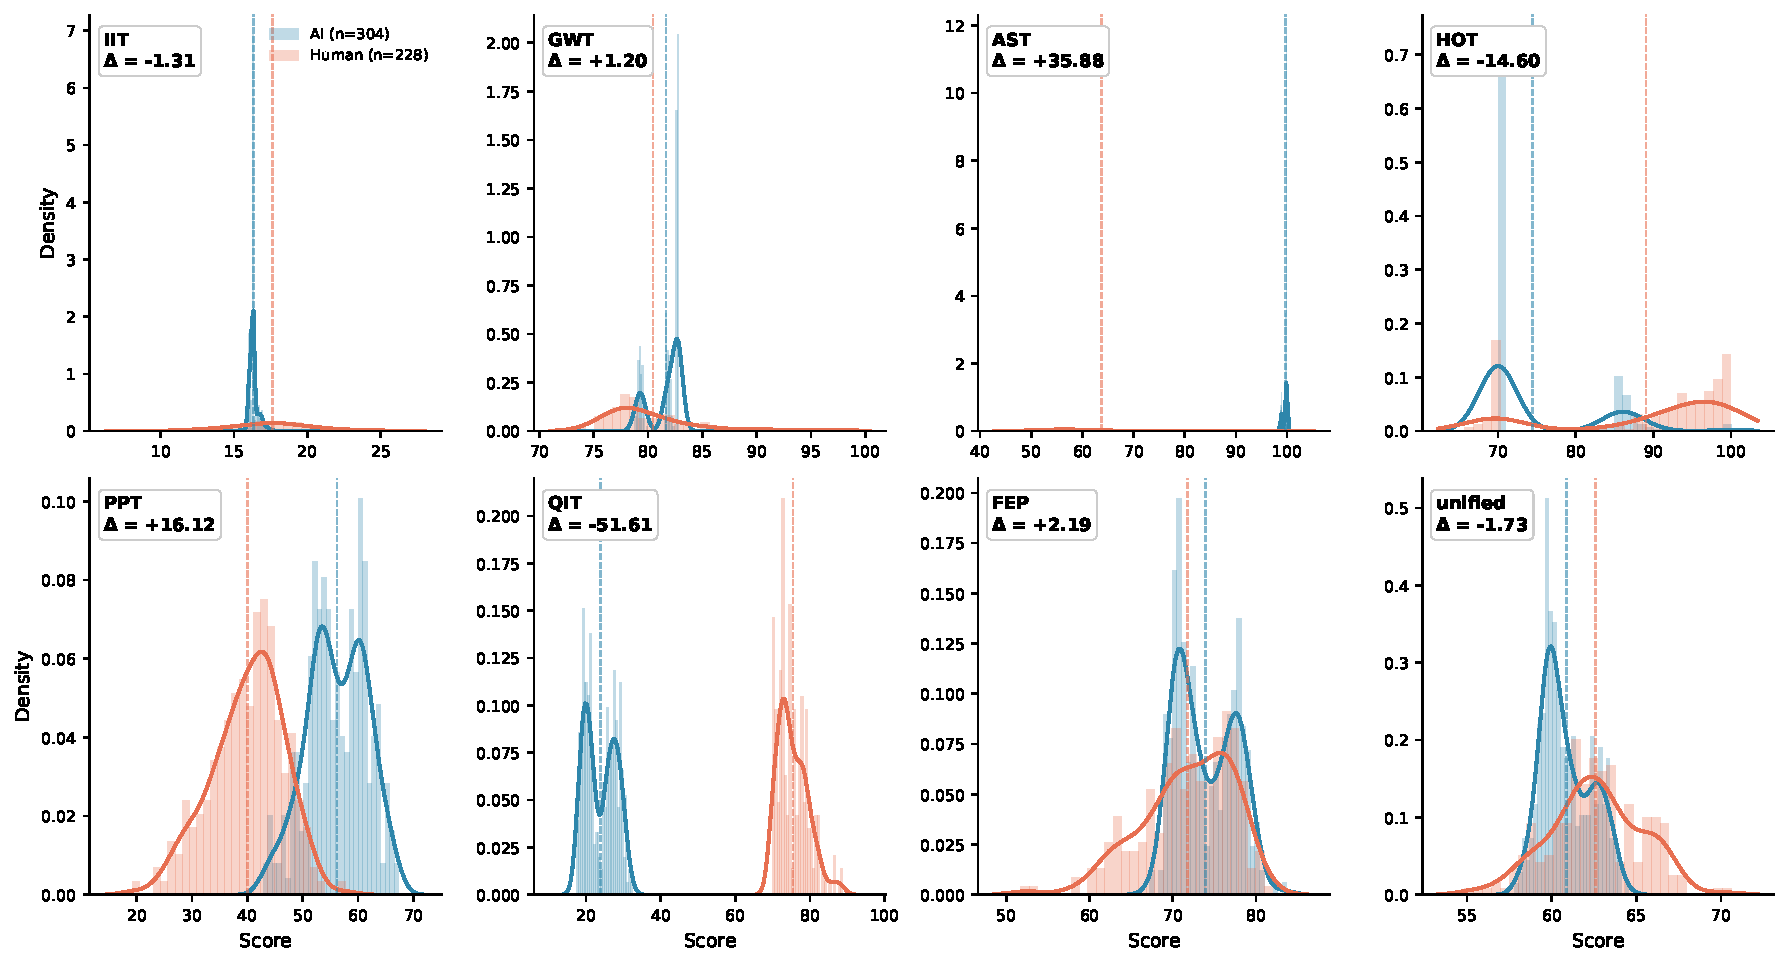
\includegraphics[width=\textwidth]{../figures/fig2_population_distributions.pdf}
\caption{Population distribution overlap for each theory. Histograms with KDE overlays of pooled AI substrate scores (teal, $n = 304$ cells) vs pooled human substrate scores (orange, $n = 228$ cells). Dashed vertical lines mark per-substrate means; $\Delta =$ AI mean $-$ human mean. IIT and GWT show sub-2-point cross-substrate gaps; FEP and the unified score also within 5 points. QIT shows the largest divergence ($\Delta = -51.6$) — AI scores collapse on long narrative stimuli where human BOLD remains in the same range.}
\label{fig:popdist}
\end{figure}

\subsection{Per-stimulus cross-substrate correlation: six of seven theories near-zero, GWT the exception}
\label{sec:results-perstim}

For each theory we compute Pearson $r$ between AI and human per-story scores under two formulations. The first averages 12 per-(model, subject) correlations; the second averages within-substrate noise then computes a single $r$:

\begin{table}[h]
\centering
\small
\begin{tabular}{lrrrc}
\toprule
\textbf{Theory} & \textbf{12-pair mean $r$} & \textbf{Model+subj.\ avg $r$} & \textbf{Permutation $p$} & \textbf{Split-half $r_1$/$r_2$} \\
\midrule
IIT             & $+0.003$ & $+0.181$ & 0.118 & $+0.31$ / $+0.10$ \\
\textbf{GWT}    & \textbf{$+0.119$} & \textbf{$+0.365$} & \textbf{0.0008} & \textbf{$+0.37$ / $+0.37$} \\
AST             & $+0.002$ & $+0.043$ & 0.718 & $+0.03$ / $+0.09$ \\
HOT             & NaN      & $+0.101$ & 0.404 & $+0.09$ / $+0.11$ \\
PPT             & $+0.031$ & $+0.038$ & 0.744 & $+0.01$ / $+0.03$ \\
QIT             & $-0.021$ & $-0.063$ & 0.583 & $-0.10$ / $+0.02$ \\
FEP             & $-0.086$ & $-0.167$ & 0.150 & $+0.02$ / $-0.31$ \\
Unified         & $-0.033$ & $-0.087$ & 0.447 & $+0.05$ / $-0.29$ \\
\bottomrule
\end{tabular}
\caption{Per-stimulus cross-substrate Pearson correlation, two formulations. Split-half stability tests use random halves of the 76 matched stories.}
\end{table}

Two findings (Figures~\ref{fig:perstim}--\ref{fig:forest}).

\paragraph{Six of seven theories show no significant cross-substrate correlation under either formulation.} Best-case $r$ magnitudes are below 0.2, permutation $p$-values are above 0.1, and split-half stability is poor for theories whose $r$ is non-negligible (e.g., IIT split halves $+0.31$ vs $+0.10$; FEP $+0.02$ vs $-0.31$). The unified-score correlation is essentially zero ($r = -0.087$, permutation $p = 0.45$). For these six theories, AI-side per-story rankings are not predictive of human-side per-story rankings --- the substrate-agnostic mathematics produces numbers that do not transfer across substrates.

\paragraph{GWT alone shows a stable cross-substrate correlation.} $r = +0.365$, permutation $p = 0.001$ (the observed correlation exceeds 99.9\% of label-shuffled null correlations), split-half correlations are nearly identical at $+0.37$ / $+0.37$. GWT's substrate-agnostic operationalization (cross-group ignition) captures stimulus-driven structure shared between AI and human substrates.

\begin{figure}[H]
\centering
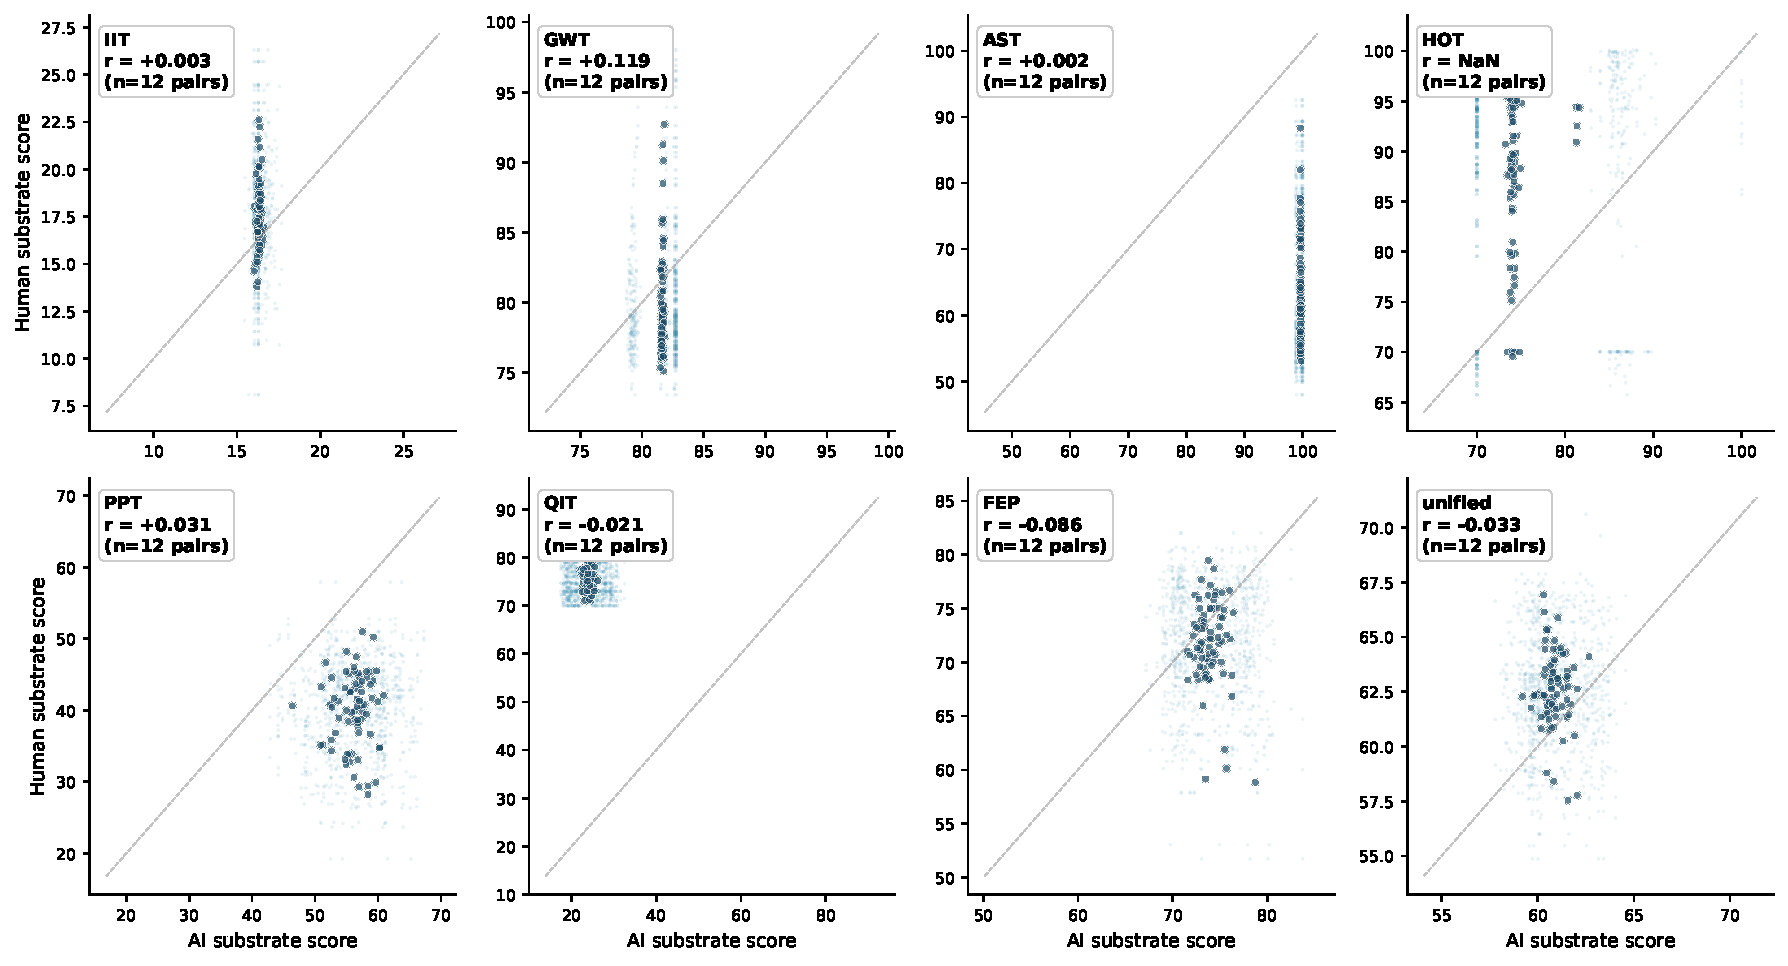
\includegraphics[width=\textwidth]{../figures/fig1_perstimulus_scatter.pdf}
\caption{Per-stimulus cross-substrate scatter for each of the seven theories plus the unified score. Each panel: AI per-story score ($x$-axis) vs human per-story score ($y$-axis); light points are individual (model, subject, story) triples, dark points are per-story means averaged across models and subjects; dashed line is identity $y = x$. Annotation: mean Pearson $r$ across 12 model-subject pairs.}
\label{fig:perstim}
\end{figure}

\begin{figure}[H]
\centering
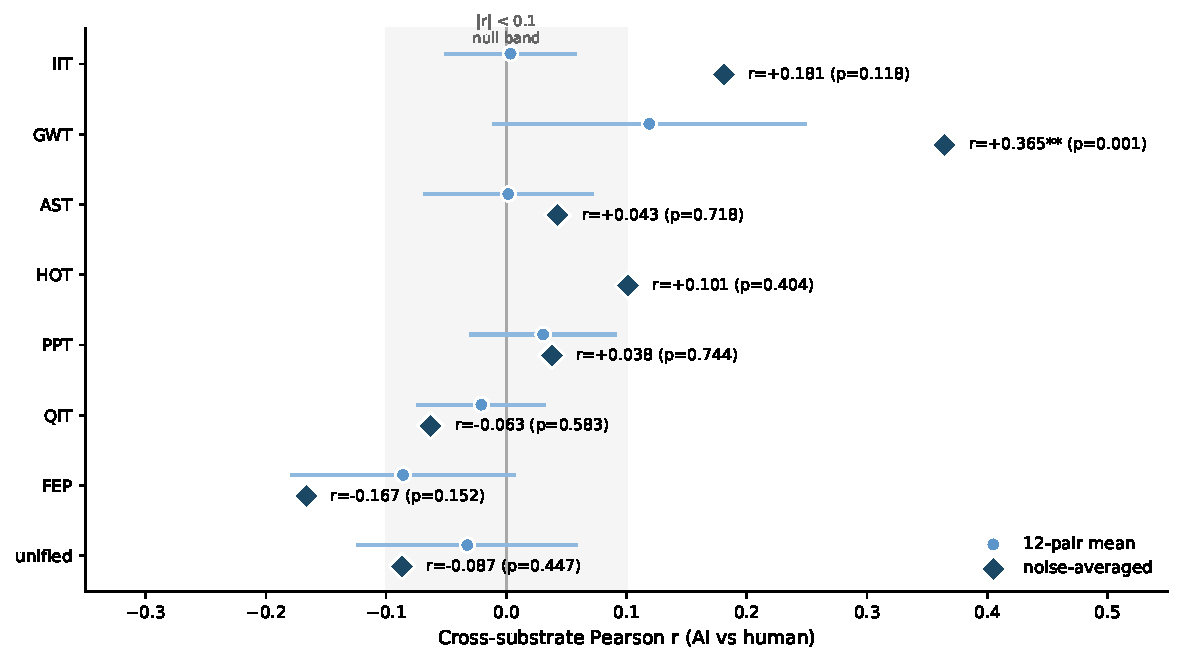
\includegraphics[width=\textwidth]{../figures/fig3_forest_correlations.pdf}
\caption{Forest plot of cross-substrate per-stimulus Pearson $r$ per theory under two formulations: the conservative 12-pair mean (left points) and the noise-averaged single-$r$ formulation (right points). Light-gray band marks $|r| < 0.1$, the conventional null-correlation region. GWT alone leaves the null band under the noise-averaged formulation.}
\label{fig:forest}
\end{figure}

\paragraph{GWT's signal is not architecturally robust,} however. Per-model breakdown (Pearson $r$ per model with subject-averaged human scores):

\begin{table}[h]
\centering
\small
\begin{tabular}{lr}
\toprule
\textbf{Model} & \textbf{GWT cross-substrate $r$} \\
\midrule
Llama 3.1 8B       & $+0.067$ \\
Phi-3 mini         & $+0.173$ \\
Mistral 7B v0.3    & $-0.185$ \\
Mistral-Nemo 12B   & $\mathbf{+0.428}$ \\
\bottomrule
\end{tabular}
\caption{GWT cross-substrate correlation per AI architecture, against subject-averaged human GWT scores across 76 stories.}
\end{table}

The signal is driven primarily by Mistral-Nemo ($+0.43$) and is absent or weakly negative on the other three architectures. The model-averaged result is robust because two of three subjects show $r > 0.30$ across all 4 models in mean-averaged comparison, but the underlying per-architecture pattern is heterogeneous. GWT is the only theory with a defensible substrate-portability claim, but the empirical evidence is consistent with the claim being architecture-conditional.

\begin{figure}[H]
\centering
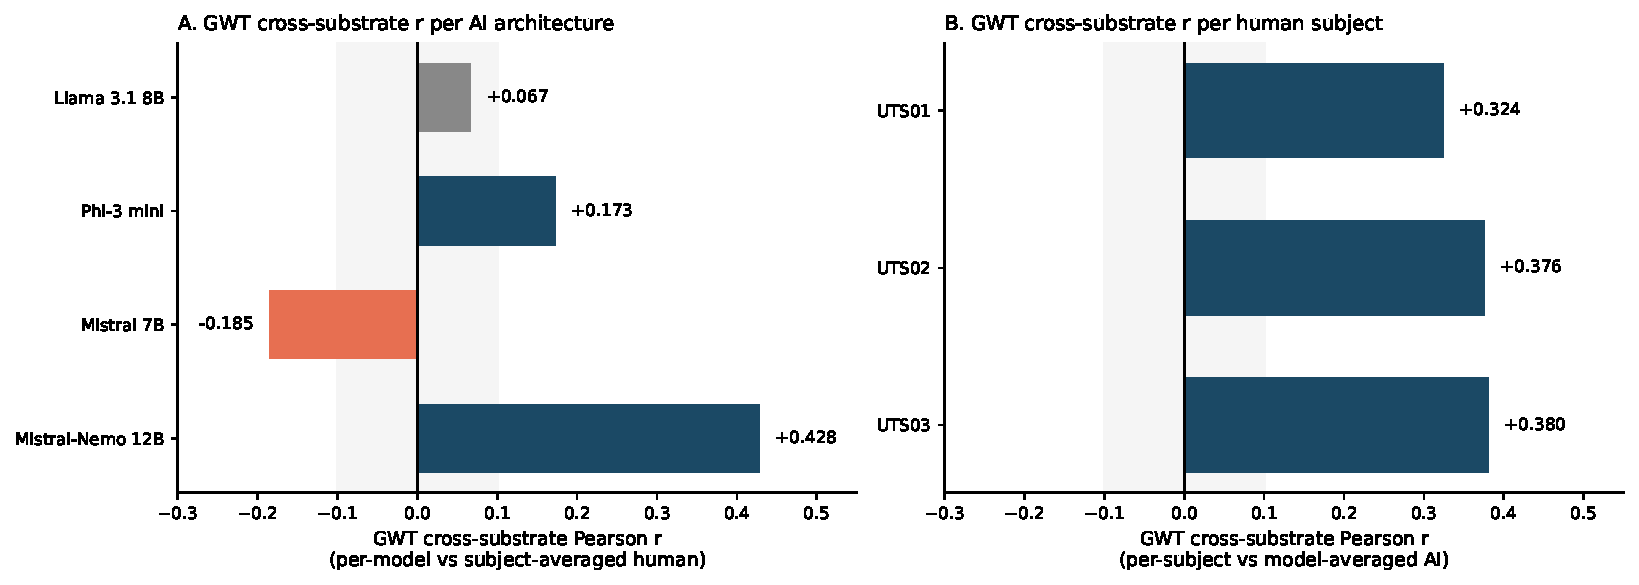
\includegraphics[width=\textwidth]{../figures/fig5_gwt_per_architecture.pdf}
\caption{GWT per-architecture cross-substrate correlation. Left panel: Pearson $r$ between each model's per-story GWT scores and subject-averaged human GWT scores. Right panel: Pearson $r$ per human subject against model-averaged AI GWT scores. The cross-subject signal is consistent (0.32--0.38); the cross-architecture signal is heterogeneous and driven by one model family.}
\label{fig:gwtarch}
\end{figure}

\subsection{AI-side variance decomposition: architecture dominates stimulus}
\label{sec:results-variance}

For each theory, we decompose AI-side per-story variance into between-story (substrate-shared candidate signal) and within-story (between-model architectural noise) components:

\begin{table}[h]
\centering
\small
\begin{tabular}{lrrcc}
\toprule
\textbf{Theory} & \textbf{Between-story SD} & \textbf{Within-story SD (model)} & \textbf{Ratio} & \textbf{Interpretation} \\
\midrule
IIT     & 0.105 & 0.255 & 0.41 & model-noise dominates \\
GWT     & 0.077 & 1.421 & 0.054 & \textbf{model-noise dominates} \\
AST     & 0.049 & 0.438 & 0.11 & model-noise dominates \\
HOT     & 1.671 & 7.293 & 0.23 & model-noise dominates \\
\textbf{PPT}     & \textbf{2.538} & \textbf{4.472} & \textbf{0.57} & \textbf{mixed} \\
QIT     & 0.833 & 3.943 & 0.21 & model-noise dominates \\
FEP     & 1.280 & 3.225 & 0.40 & model-noise dominates \\
Unified & 0.588 & 1.308 & 0.45 & model-noise dominates \\
\bottomrule
\end{tabular}
\caption{AI-side variance decomposition. Between-story SD = standard deviation of per-story mean scores; within-story SD = mean across stories of within-story SD (across the 4 models). Ratio $< 1$ indicates architectural noise dominates stimulus signal.}
\end{table}

For seven of eight theories (the seven plus unified), between-story variance on the AI side is smaller --- typically much smaller --- than between-model variance for the same story (Figure~\ref{fig:vardecomp}). AI substrate per-story differentiation is dominated by \emph{which model is running}, not by \emph{which story is being processed}. Only PPT approaches a mixed regime (ratio 0.57); for the other six theories, model-noise exceeds stimulus signal by factors of $2\times$ to $18\times$.

\begin{figure}[H]
\centering
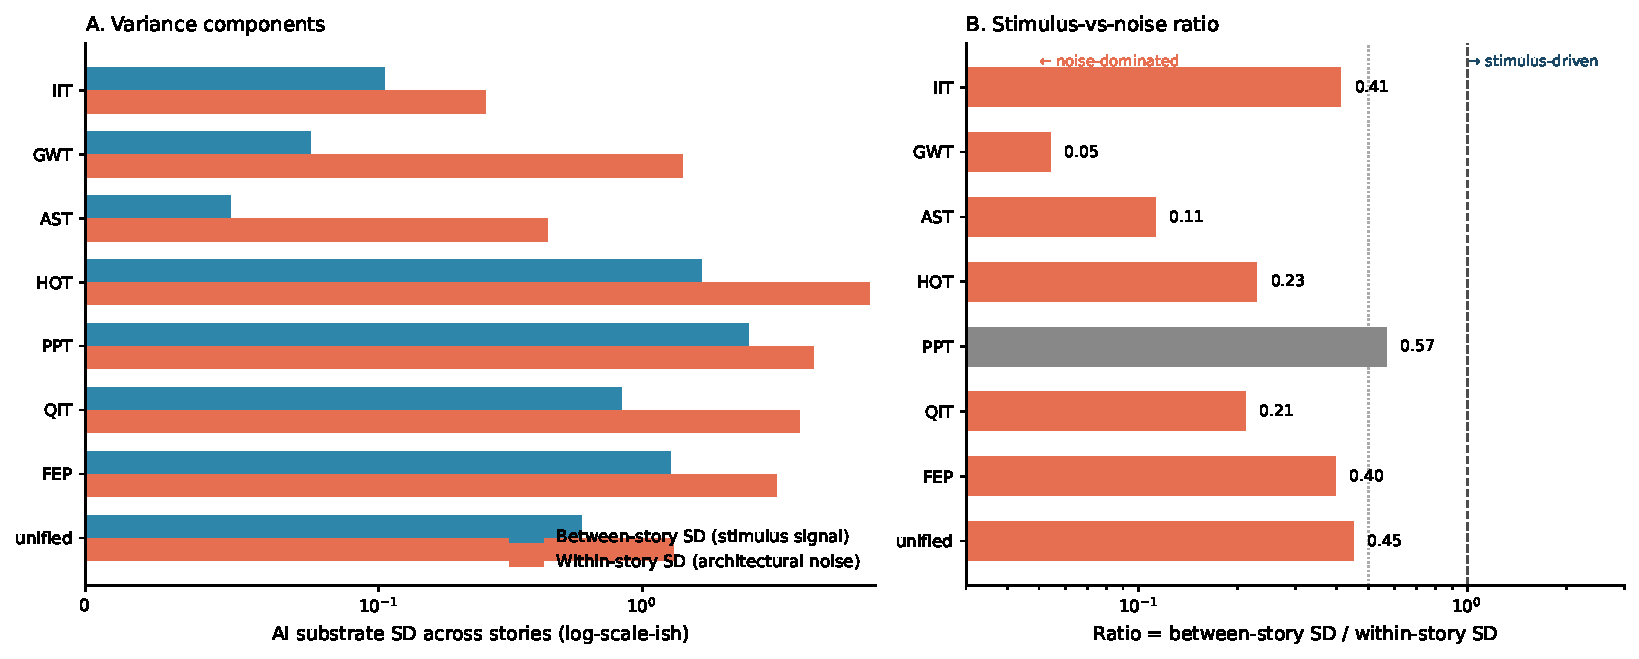
\includegraphics[width=\textwidth]{../figures/fig4_variance_decomposition.pdf}
\caption{AI-side variance decomposition per theory. Left: between-story SD (stimulus-driven signal) vs within-story SD (between-model architectural noise) for each theory. Right: ratio of the two. Theories left of the dashed unity line have architectural noise dominating stimulus signal. Six of seven theories cluster well below the line.}
\label{fig:vardecomp}
\end{figure}

Two of the variance-ratio entries are confounded with operationalization saturation and should be interpreted cautiously. AST's between-story SD on the AI side is 0.049 --- but the AI mean is 99.64 (sd 0.45) across all cells, indicating the AST operationalization is at the numerical ceiling. The ``low between-story variance'' reflects ceiling saturation, not necessarily an architectural-noise-dominates conclusion. Similarly, HOT's per-story SD reflects the 70.00 floor for two of four models (constant output regardless of stimulus). The variance-ratio interpretation is most reliable for the five non-saturated theories (IIT, GWT, PPT, QIT, FEP); for AST and HOT, the ratio is consistent with architectural-noise-dominance but also with operationalization-ceiling-saturation as the proximate cause.

GWT --- the only theory showing detectable cross-substrate correlation --- has the \emph{lowest} variance ratio (0.054), the most extreme architectural noise dominance. Its substrate-shared signal is detectable despite this because the small between-story component aligns with human between-story variation. GWT's AI-side stimulus-relevant variance is detectable but small; the other theories' AI-side outputs do not contain enough stimulus-relevant variance to compare against human stimulus-relevant variance at all.

The variance decomposition explains the population magnitude alignment observed in \S\ref{sec:results-population}. Each AI architecture produces a model-specific mean theory score, and those means happen to fall in overlapping range with the human mean for some theories. The ``magnitude alignment'' of IIT (gap $-1.3$), GWT (gap $+1.2$), FEP (gap $+2.2$), and unified (gap $-1.7$) is coincidental: it reflects the AI's architectural mean scores landing near the human stimulus-averaged mean score. The four remaining theories (AST, HOT, PPT, QIT) show large gaps that the architectural-noise floor cannot explain by coincidence alone --- the operationalizations produce systematically different output ranges across substrates.

\subsection{Geometric integration: per-substrate consensus and unified-score robustness}
\label{sec:results-geometric}

We apply the Fisher-Rao geometric integration (\S2.5) to all 532 matched-corpus (substrate, stimulus) cells: 4 models $\times$ 76 stories $= 304$ AI cells and 3 subjects $\times$ 76 stories $= 228$ human cells. Per-substrate distribution analysis pools across cells within each substrate; cross-substrate per-stimulus correlation averages AI scores across the 4 models and human scores across the 3 subjects per story (as in \S\ref{sec:results-population} and \S\ref{sec:results-perstim}).

\paragraph{Per-substrate distributions:}

\begin{table}[h]
\centering
\small
\begin{tabular}{lrrrr}
\toprule
\textbf{Field} & \textbf{AI mean (sd)} & \textbf{Human mean (sd)} & \textbf{Gap} & \textbf{KS $p$} \\
\midrule
Naive unified           & 60.86 (1.45)  & 62.59 (2.71)  & $-1.73$ & $<$ .001 \\
Riemannian unified      & 70.77 (2.24)  & 68.92 (2.44)  & $+1.86$ & $<$ .001 \\
Theoretical consensus   & 0.357 (0.003) & 0.372 (0.009) & $-0.015$ & $<$ .001 \\
Geometric coherence     & 0.549 (0.019) & 0.550 (0.021) & $-0.000$ & .087 \\
\bottomrule
\end{tabular}
\caption{Per-substrate distributions of geometric integration outputs.}
\end{table}

\paragraph{Two changes between naive and Riemannian integration.} First, both produce a non-significant near-zero cross-substrate per-stimulus Pearson $r$: naive $r = -0.087$ ($p = 0.46$, permutation); Riemannian $r = -0.185$ ($p = 0.11$). The null cross-substrate correlation is preserved under the more rigorous integration. Second, the Riemannian $r$ is about twice as negative in magnitude as the naive $r$, and the substrate magnitude gap reverses sign: under the naive arithmetic mean the human substrate scores higher on average (AI $-$ human $= -1.73$), under the Riemannian mean the AI substrate scores higher (AI $-$ human $= +1.86$). Both unified-score means also shift upward by 7--10 points under the geometric integration (AI: 60.86 $\rightarrow$ 70.77; Human: 62.59 $\rightarrow$ 68.92), a consequence of the probability-logit transform in step 5 of \S2.5. The null cross-substrate correlation is robust to integration method; the magnitude direction is not.

\paragraph{Prior-matrix sensitivity.} The geometric integration uses a literature-based $7 \times 7$ theoretical-compatibility prior matrix (\S2.5). To verify the Riemannian $r$ is not an artifact of this hand-encoded prior, we re-ran the integration under three alternative priors: uniform 0.5 matrix (all theory pairs equally compatible), identity matrix (no inter-theory influence), and 20 random perturbations (each off-diagonal cell $\sim$ Uniform$[0.3, 0.95]$). The Riemannian cross-substrate $r$ remained in the narrow range $[-0.213, -0.163]$ across all priors (mean $-0.184$, sd 0.011 over the 20 random matrices). The literature-based prior produces the same conclusion as any reasonable alternative; the matrix is not driving the result.

\paragraph{A modest consensus offset, of unclear substantive importance.} Per-substrate theoretical consensus distributes as AI: 0.357 $\pm$ 0.003; Human: 0.372 $\pm$ 0.009 --- a gap of 0.015 on a 0--1 scale (4\% relative). The KS test of distribution equality is significant at $p < .001$, but consistent with \S\ref{sec:results-population}'s caveat about KS at this sample size ($n_{\mathrm{AI}} = 304$, $n_{\mathrm{human}} = 228$), this significance is uninformative about magnitude. We report the offset for completeness: humans' 7-theory rankings have slightly tighter within-cell agreement than AI's. The substantive magnitude of this offset is small relative to the cell-to-cell noise (AI sd 0.003), and we do not interpret it as a primary cross-substrate finding. It is consistent with --- but not strong independent evidence for --- the variance-decomposition observation in \S\ref{sec:results-variance} that AI theories produce architecturally-idiosyncratic per-story scores.

\paragraph{Curvature output is degenerate.} The geometric integration's manifold-curvature output saturates at the numerical lower bound ($\tanh(-\infty) = -1$) on both substrates, with cross-cell range of order $10^{-4}$. The non-zero cross-substrate correlation reported by automated analysis ($-0.243$, $p = 0.034$) is therefore floating-point noise on a saturated quantity and is not interpretable. See \S\ref{sec:limitations}.

\begin{figure}[H]
\centering
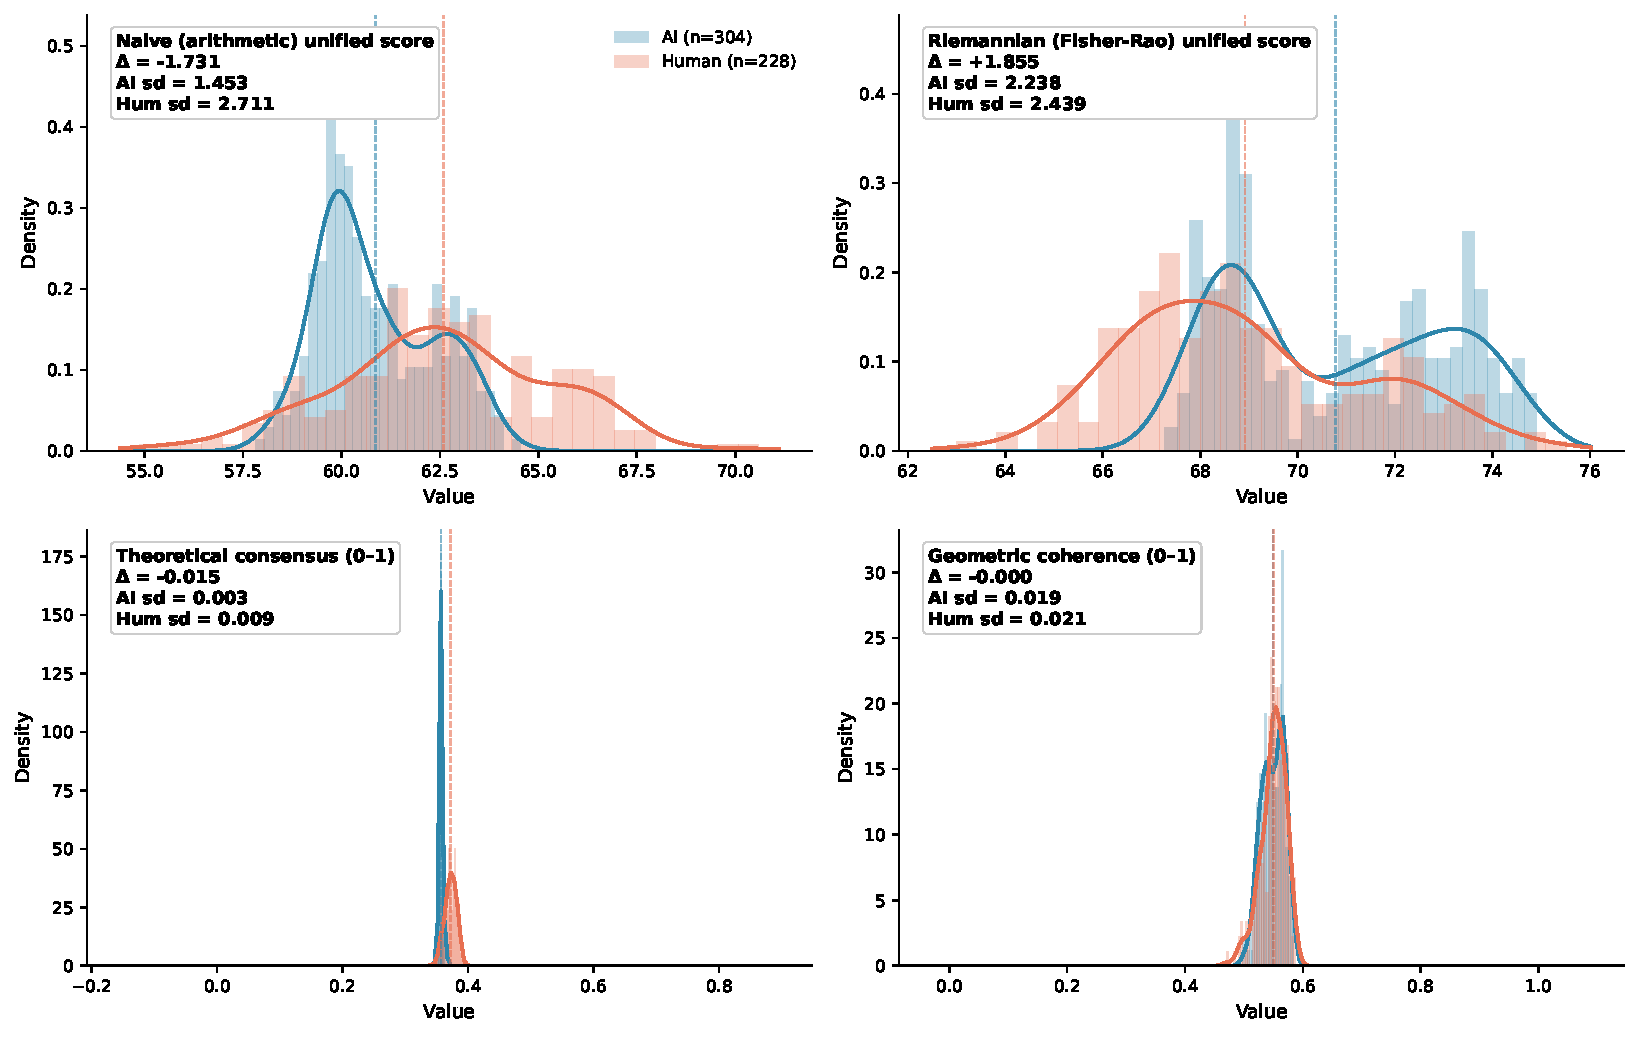
\includegraphics[width=\textwidth]{../figures/fig6_geometric_integration.pdf}
\caption{Fisher-Rao geometric integration: per-substrate distributions. Top row: naive (arithmetic) vs Riemannian (Fisher-Rao) unified scores. Bottom row: theoretical consensus and geometric coherence. Both unified-score formulations yield near-zero cross-substrate correlation. Humans show slightly higher within-substrate theoretical consensus than AI ($\Delta = -0.015$, KS $p < .001$ --- significance is uninformative at $n = 532$; magnitude is small).}
\label{fig:geomint}
\end{figure}

\subsection{Per-model summary}

For completeness, per-model unified-score statistics on the LeBel set:

\begin{table}[h]
\centering
\small
\begin{tabular}{lrrrl}
\toprule
\textbf{Model} & \textbf{$n$ stories} & \textbf{Unified mean (sd)} & \textbf{HOT mean (sd)} & \textbf{Notes} \\
\midrule
Llama 3.1 8B        & 81 & 60.56 (0.79) & 70.00 (0.00) & HOT saturated \\
Mistral 7B v0.3     & 81 & 60.37 (1.08) & 70.00 (0.00) & HOT saturated \\
Mistral-Nemo 12B    & 81 & 59.82 (1.21) & 71.48 (6.49) & HOT near-saturated \\
Phi-3 mini          & 81 & 62.76 (0.66) & 86.34 (1.63) & HOT non-saturated \\
\bottomrule
\end{tabular}
\caption{Per-model unified- and HOT-score statistics. Per-model $n$ is 81 (AI-side dataset before matching with the human substrate's 76-story set); the cross-substrate analyses in \S\ref{sec:results-population}, \S\ref{sec:results-perstim}, \S\ref{sec:results-variance} use the matched $n = 76$ throughout.}
\end{table}

Two of four models produce a constant HOT $= 70.00$ across all 81 stories: the HOT operationalization (cross-region canonical correlation) is saturated and stimulus-invariant on these models. This is consistent with the broader variance-decomposition pattern: AI-side theory scores are dominated by architectural structure, and for HOT specifically that structure is so dominant that two architectures produce identical scalars regardless of input.

\section{Discussion}

\subsection{Magnitude overlap reflects variance-source coincidence, not measurement concordance}

Prior exploratory work comparing humans and AI on behavioral approximations of these seven theories had found that the populations score in overlapping ranges, leading to the interpretation that mathematical consciousness theories cannot discriminate conscious from non-conscious systems. The population-level substrate analysis (\S\ref{sec:results-population}) shows AI distributions overlapping human distributions for IIT, GWT, FEP, and the unified score --- partially consistent with the prior magnitude-overlap finding, though four theories (AST, HOT, PPT, QIT) show substantial cross-substrate divergence.

The variance decomposition (\S\ref{sec:results-variance}) and per-stimulus correlation (\S\ref{sec:results-perstim}) revise the interpretation of that overlap. The ``no-discrimination'' reading assumes both substrates produce stimulus-relevant scores, which then happen to align. The data show something different:

\begin{itemize}
  \item The human substrate produces stimulus-relevant scores: between-story variance reflects what story is being processed.
  \item The AI substrate produces architecture-relevant scores: between-story variance is smaller than between-model variance for six of seven theories. AI per-story differentiation reflects \emph{which model is running}, not \emph{which story is being processed}.
\end{itemize}

The ``alignment'' of AI mean and human mean is consistent with coincidental overlap of two fundamentally different variance sources. Each AI architecture has an architecture-specific mean theory score; the four architectures' means fall in the same range as the human stimulus-averaged mean. The magnitude overlap is not informative evidence \emph{for} substrate-shared signal, since the AI-side variance is dominated by architectural identity rather than stimulus content. The data do not rule out shared signal, however --- only that magnitude overlap on its own does not establish it.

Mathematical consciousness theories, as currently operationalized, cannot serve as cross-substrate consciousness discriminators on transformer substrates. The theories' AI-side outputs are not detectable measurements \emph{of the AI's stimulus processing} --- whether because no such measurement exists in the activations or because these operationalizations cannot resolve it through the architectural noise. Both possibilities are open and are discussed in \S\ref{sec:discussion-six}. Either way, the operationalizations do not deliver substrate-portable measurements for six of the seven theories.

\subsection{GWT is a genuine partial exception}

Global Workspace Theory's cross-group ignition operationalization is the only one of the seven that produces stimulus-relevant AI-side signal sufficient to detect cross-substrate correlation. After averaging within-substrate noise, GWT shows $r = +0.365$ (permutation $p = 0.001$, split-half $+0.37$/$+0.37$). The signal is consistent across all three human subjects (per-subject $r$: 0.32, 0.38, 0.38). This is a defensible claim that GWT's substrate-agnostic operationalization captures stimulus-driven structure shared between transformer attention dynamics and human BOLD signals.

Three caveats matter:

First, GWT's AI-side variance is overwhelmingly architectural --- between-model SD $= 1.42$ vs between-story SD $= 0.077$, an $18\times$ ratio. The cross-substrate-shared signal exists but is a tiny fraction of total AI-side variance. The fact that this small signal is detectable means GWT operationalizes something stimulus-relevant; the fact that it is small means the signal is fragile to architectural perturbation.

Second, per-architecture breakdown reveals heterogeneity. Mistral-Nemo shows $r = +0.43$; Mistral 7B shows $r = -0.19$. The three other architectures cluster near zero. The model-averaged result is driven primarily by Mistral-Nemo. This is consistent with several interpretations: (a) Mistral-Nemo's attention dynamics genuinely process narrative structure in a way that correlates with human BOLD, while other architectures do not; (b) Mistral-Nemo has a particular implementation quirk (e.g., its 128k-context-capable attention pattern) that incidentally aligns with human stimulus processing; (c) the across-architecture variation is statistical noise at our $n$.

Third, GWT is the theory whose operationalization is most behaviorally evocative (``global broadcast'') and the operationalization most directly inherits from a theory framed in terms of cognitive-access architecture. It is therefore the theory most plausibly tied to substrate features (cross-group information mixing) that both transformers and brains might share for reasons unrelated to consciousness. A positive GWT cross-substrate correlation is consistent with both ``GWT captures a real substrate-shared computational property'' and ``GWT operationalizes a cross-group-mixing quantity that both transformers and brains happen to exhibit on narrative input for non-consciousness-related reasons.'' Distinguishing these requires further analyses we do not undertake here.

\subsection{Why six theories produce stimulus-insensitive AI outputs}
\label{sec:discussion-six}

For six of seven theories, the AI substrate's between-story SD is a small fraction of within-story (between-model) SD. The substrate-agnostic operationalizations, when run on transformer attention activations, produce outputs that vary across architectures but barely vary across stories within a fixed architecture.

This is not a generic statement about transformers being insensitive to stimuli --- transformers are demonstrably sensitive to stimuli, since their \emph{outputs} (generated text, logits) clearly differ across inputs. The variance-decomposition finding is specific to the \emph{attention-mass aggregation} the theory operationalizations consume. When the substrate-agnostic operationalizations summarize transformer attention into the ($T$, $N$) activity matrix and then compute integrated-information / global-broadcast / canonical-correlation / etc., the summary discards most of the stimulus-driven information that the transformer's downstream computation uses, retaining mostly architectural structure.

This suggests two non-exclusive possibilities:

\paragraph{(I) The standard operationalizations are not the right operationalizations.} Different substrate-agnostic implementations of the same seven theories --- using different transformer activations (e.g., MLP outputs, residual stream norms), different aggregations (per-head vs per-layer vs per-token), or different score formulas --- might recover stimulus-relevant AI signal. The negative finding is contingent on our specific operationalization choices.

\paragraph{(II) The theories' substrate-level claims are vacuous for current AI substrates.} The substrate-independence claim of contemporary consciousness theory requires the theories to identify substrate-portable structure. If the AI substrate's attention dynamics, summarized in the standard ways, do not carry stimulus-relevant signal that the theories can detect, then the theories' substrate-level claims are not testable on these substrates with these operationalizations. The theories may apply elsewhere (e.g., to spiking networks, to recurrent architectures), but for transformer activations as standardly summarized, there is no stimulus-driven signal to which the theories' substrate-agnostic operationalizations attach.

Distinguishing (I) and (II) requires either developing new operationalizations or applying the existing ones to substrates where stimulus-driven AI variance is more pronounced. Both directions are open.

\subsection{Scope of the result}

The negative result here applies to one class of mathematical operationalizations, one stimulus regime, and a sample of four AI architectures. It does not establish that AI is not conscious or that humans are; it does not establish that any of the seven theories is wrong about consciousness; it does not establish that no alternative operationalization (e.g., on MLP outputs or residual-stream norms), substrate summarization, or stimulus regime could succeed; and it does not establish that AI cannot be tested for consciousness in any sense. The analyses measure operationalizations, not consciousness.

What is established: when seven leading mathematical consciousness theories are substrate-agnostically operationalized in the most natural way and applied identically to AI attention activations and human BOLD signals on the same naturalistic stimuli, six of seven theories produce AI-side outputs whose per-story variance is dominated by architectural rather than stimulus-driven sources. The population magnitude alignment across substrates is consistent with coincidental overlap of architectural-noise and stimulus-driven variance. The substrate-independence claim of contemporary consciousness theory, as standardly operationalized, is not testable on transformer substrates with naturalistic narrative stimuli using these operationalizations: no AI-side stimulus-driven measurement of sufficient signal-to-noise is available to compare against the human-side measurement. GWT is the only theory among the seven with even tentative empirical support for a substrate-portability claim, and that support is contingent on a single AI architecture among the four tested.

\section{Limitations}
\label{sec:limitations}

\paragraph{Stimulus modality asymmetry.} Humans hear continuous audio (Moth Radio Hour recordings --- voice, prosody, timing, emotional inflection); AI reads truncated text. Any theory sensitive to paralinguistic content measures genuinely different stimuli on the two substrates. This is a fundamental cross-substrate asymmetry and may itself contribute to the per-story-correlation null results for theories whose operationalization is more perceptual than linguistic.

\paragraph{Token truncation.} AI inputs were truncated to 1500 tokens, $\sim$37\% of the median full-story length ($\sim$4000 tokens). Larger context windows might engage qualitatively different attention patterns. The 70B-class models would not fit at 1500-token context on 2 $\times$ 80 GB GPU and were excluded; smaller models provide architectural breadth but not scale breadth.

\paragraph{Subject sample.} Three human subjects provides stable per-subject substrate signatures but modest population breadth. The full LeBel dataset has eight subjects; including the remaining five would not change the qualitative result but would tighten estimates.

\paragraph{Voxel-to-parcel reduction.} $K$-means parcellation of $\sim$81{,}000 voxels to 200 parcels per (subject, story) re-clusters fresh each time, sacrificing cross-story parcel comparability for within-story signal-to-noise. A theory whose substrate signature lives at fine spatial resolution is invisible to this analysis.

\paragraph{Per-(subject, story) parcellation, not joint.} Each (subject, story) BOLD is $K$-means clustered independently. Parcels are therefore not the same parcels across subjects or across stories. This is a design choice favoring substrate-method symmetry (both AI and human substrates do clustering-based aggregation) over cross-subject parcel-comparability. Cross-subject correlation in our analyses is at the per-story-scalar level, not parcel level.

\paragraph{IIT bipartition search uses stratified sampling on both substrates.} $\Phi$ uses Normalized Cut with exhaustive enumeration of bipartitions for groups of $N \leq 8$ nodes and stratified sampling for $N > 8$. Transformer per-layer groups have 32 heads; fMRI per-network groups have $\sim$20 parcels --- both above the enumeration threshold, both use sampling. The stratified sample is seeded identically across substrates ($\text{seed} = 42$), so the algorithmic surface is the same. The exhaustive-enumeration regime is never hit by either substrate at our group sizes; what this means substantively is that IIT $\Phi$ as reported here is a Monte Carlo estimate of the true minimum bipartition, with sampling variance that we do not formally bound.

\paragraph{Temporal-axis units differ across substrates.} The $T$ dimension of the activity matrix is tokens on the AI side ($T \approx 1500$ per story) and sentences on the human side ($T \approx 10$--$50$ per story). The seven theory calculators operate on $(T, N)$ matrices without unit awareness, which is the source of their substrate portability. But theories whose output depends on temporal pattern --- PPT (prediction-error trajectory), FEP (cross-entropy series), and QIT (long-range mutual information at distances $d \in \{1, 3, 5, 10\}$ on the $T$ axis) --- are measuring quantities at very different time scales on the two substrates. The same nominal distance $d = 10$ means ``10 tokens later'' on the AI side and ``10 sentences later'' on the human side. The paper's cross-substrate comparisons treat these as the same; they are not, and any non-zero cross-substrate signal in PPT/FEP/QIT could partly reflect this unit-scale mismatch rather than substrate-shared computation.

\paragraph{AR(1) vs LLM-logits prediction-adapter asymmetry.} PPT and FEP rest on the comparability of an AR(1) regression's residuals and a transformer's next-token logit entropy. These are not equivalent prediction models. PPT and FEP results should be interpreted as comparing operationalization choices made for substrate-comparability, not as comparing equivalent prediction architectures.

\paragraph{PPT and FEP cross-substrate scores are partly uninterpretable, not informative nulls.} The asymmetry above is sharper than a difference in predictor strength. PPT and FEP both depend on prediction-distribution entropy and prediction-error quantities. The transformer prediction adapter (\S\ref{sec:adapters}) computes the differential entropy of the next-token logit distribution --- a probability-distribution entropy over a generative model. The fMRI prediction adapter (\S\ref{sec:adapters}) reports a leverage-normalized magnitude of the AR(1)-predicted value, $\log_+(|\hat{x}_t| / \sigma_{\text{residual}})$, which is a magnitude scalar in different units; it is not differential entropy of any distribution. The two adapters therefore do not report the same kind of quantity, only a quantity that occupies the same role in the formula. PPT and FEP cross-substrate scores aggregate substrate-specific operationalization choices and substrate-agnostic theory portability into a single null, and the present analysis cannot identify which contribution dominates. PPT and FEP cross-substrate nulls should be read as uninterpretable rather than as evidence against substrate-portability of either theory.

\paragraph{HOT operationalization saturation.} Cross-region canonical correlation produces a constant HOT $= 70.00$ across all stories for two of four AI models. This is a finding about transformer information geometry (the cross-group representational-similarity quantity is stimulus-invariant on these architectures) but reduces effective statistical power for HOT specifically.

\paragraph{AST operationalization ceiling.} AST produces a near-constant 99.64 (sd 0.45) across all AI models and stories. Self-prediction at the cross-group level is saturated on transformer attention. Like HOT, this is itself a finding but precludes a proper per-stimulus correlation test for AST.

\paragraph{QIT spatial-separation transferability.} QIT's substrate-agnostic operationalization weights mutual information by node-index separation. Node index in transformers reflects head/layer ordinal; node index in fMRI reflects $K$-means cluster ID. Neither is a true spatial coordinate. The same QIT calculator on the two substrates uses the same scalar quantity but the meaning of ``separation'' differs.

\paragraph{Per-model heterogeneity in GWT.} GWT's cross-substrate correlation is driven primarily by Mistral-Nemo. Replication across additional architectures (especially larger and structurally different ones --- Mixtral, Gemma, Olmo) is needed before the cross-substrate-shared signal can be claimed as architecture-general.

\paragraph{Multiple-comparison correction.} We report 7 theories $\times$ 12 model-subject pairs $= 84$ per-pair correlations and 8 model-and-subject-averaged correlations (one per theory + unified). No formal multiple-comparison correction is applied. GWT's permutation $p = 0.0008$ survives Bonferroni correction at 7 tests ($\alpha = 0.007$); the other correlations would not have survived even uncorrected.

\paragraph{Non-independence of model-subject pairs.} Each of the 12 model-subject pairs shares a model with 3 other pairs and a subject with 4 other pairs. The mean and SD of the 12 $r$-values reported in \S\ref{sec:results-perstim} should not be treated as 12 independent samples. The model-and-subject-averaged formulation in \S\ref{sec:results-perstim} avoids this issue by collapsing to one $r$ per theory.

\paragraph{One $\Phi$ approximation, one parcellation method, one stimulus dataset.} Each is a methodological choice; alternatives might produce different findings.

\paragraph{Geometric integration manifold-curvature saturation.} The information-geometric integration's manifold-curvature output saturates at the numerical lower bound ($\tanh(-\infty) = -1$) on both substrates, with cross-cell range of order $10^{-4}$. This is a property of the specific manifold-coordinate construction we adopt (per-theory coordinates with off-diagonal compatibility-weighted influences) and the resulting near-singular metric tensor determinant. The other geometric outputs (Riemannian unified, theoretical consensus, geometric coherence) have meaningful spread and are interpreted normatively; curvature is reported for completeness but is not analytically informative in this implementation. An alternative manifold-coordinate construction might restore non-saturated curvature; we have not explored this.

\paragraph{Theoretical-compatibility prior in geometric integration.} The literature-based $7 \times 7$ theoretical-compatibility matrix used in geometric integration is fixed and hand-encoded. Different priors (e.g., learned from data, or based on different theory-comparison literature) would shift the dynamic weights and could affect the Riemannian unified score. We hold the prior constant across substrates and stimuli; cross-substrate analyses are therefore not confounded by prior-substrate interactions, but the absolute Riemannian-unified scores depend on the prior choice. The cross-substrate $r$ is robust to prior choice (\S\ref{sec:results-geometric} sensitivity analysis: range $[-0.21, -0.16]$ across uniform, identity, and 20 random alternative priors), but other Riemannian outputs (specifically the dynamic-weight distributions and the absolute Riemannian unified-score means) are not invariant to the prior and should be interpreted as conditional on it.

\paragraph{No simultaneous AI/human stimulus exposure.} AI and human substrates were processed at different times. Stimulus order, attentional state, and task framing are not controlled cross-substrate. Human subjects passively listened; AI substrates received text without explicit task framing.

\section{Conclusion}

We tested whether substrate-agnostic operationalizations of seven mathematical consciousness theories produce concordant measurements when applied identically to AI transformer activations and human fMRI BOLD signals on the same narrative stimuli. The empirical result, in three parts:

\begin{enumerate}
  \item Population-level magnitudes overlap between AI and human substrates for four of seven (plus unified) --- unified-score gap $-1.7$ on a 0--100 scale; three theories (IIT, GWT, FEP) under 5-point gaps. Four theories (AST, HOT, PPT, QIT) show substantial cross-substrate divergence.
  \item Per-stimulus rankings: six of seven theories produce essentially zero cross-substrate correlation (Pearson $r \in [-0.17, +0.18]$ after noise averaging). Global Workspace Theory is the exception with a model-and-subject-averaged $r = +0.365$ ($p = 0.001$), though the per-architecture breakdown is heterogeneous ($r$ in $[-0.19, +0.43]$) and consistent with the across-architecture pattern being noise at $n = 4$ architectures.
  \item The AI substrate's per-story variance is dominated by architectural rather than stimulus-driven sources for six of seven theories. The population magnitude alignment is therefore consistent with coincidental overlap of architecturally-driven AI variance and stimulus-driven human variance, but the data do not exclude the alternative that substrate-shared signal is present but invisible to these operationalizations.
\end{enumerate}

Robustness checks: Fisher-Rao information-geometric integration preserves the null cross-substrate correlation (Riemannian-mean $r = -0.185$, n.s.), reverses the sign of the magnitude gap (AI higher under Riemannian, humans higher under naive), and sharpens the cross-substrate $r$ in the negative direction. The Riemannian $r$ is stable across alternative compatibility-prior matrices (uniform, identity, 20 random perturbations all yield $r$ in $[-0.21, -0.16]$). A modest per-substrate consensus offset (AI 0.357 vs Human 0.372 on a 0--1 scale) is consistent with the variance decomposition; its substantive importance is small relative to within-cell noise and is not promoted to a primary finding.

These substrate-agnostic operationalizations do not produce empirically meaningful cross-substrate measurements on transformer substrates: the AI-side operationalizations fail to produce detectable stimulus-relevant signal --- whether because no such signal exists in the activations or because the operationalizations cannot resolve it through architectural noise. The substrate-independence claim, on this evidence, is not testable on transformer substrates via these operationalizations on naturalistic narrative stimuli.

GWT is the partial exception. Its operationalization (cross-group ignition / global broadcast) produces stimulus-relevant AI-side signal in some architectures and that signal modestly correlates with human stimulus-relevant signal across subjects. GWT is therefore the only theory of the seven for which a substrate-portability claim has tentative empirical support. Whether GWT's cross-substrate signal indexes consciousness-related processing or some non-consciousness-related substrate property both brains and transformers happen to exhibit is an open question.

The methodological framework --- the \texttt{Substrate} abstraction, the substrate-agnostic operationalizations, the open-source reproduction pipeline --- survives the empirical result and is released for future cross-substrate consciousness comparisons. Subsequent work may identify operationalizations or substrate-aggregation choices that recover stimulus-relevant AI signal for the six near-null theories, or may establish that GWT's cross-substrate signal generalizes (or fails to) across additional architectures and stimulus regimes. Either direction sharpens the empirical conversation about consciousness-as-mathematics in ways that magnitude-only comparisons cannot.

\section*{Data Availability}

All code, data, and analysis scripts are released at \url{https://github.com/devmance/SEMCA} under MIT license. The repository contains the substrate abstraction, theory calculators, runners, and pre-computed substrate scores for all (model, story) and (subject, story) cells reported in this paper.

The LeBel ds003020 raw dataset is on OpenNeuro under CC0 license; preprocessing scripts in this repository reproduce the BOLD-extracted activity matrices.

\section*{Acknowledgments}

Compute provided by Lambda (lambda.ai, 2 $\times$ H100 80 GB SXM5). Open-weight models from Meta, Mistral AI, Microsoft. fMRI data from \citet{lebel2023natural} --- the Moth Radio Hour collection.

\clearpage
\clearpage
\bibliographystyle{plainnat}
\bibliography{refs}

\end{document}
